\documentclass{beamer}

\mode<presentation>
{
  \usetheme{CambridgeUS}      % or try Darmstadt, Madrid, Warsaw, ...
  \usecolortheme{default} % or try albatross, beaver, crane, ...
  \usefonttheme{default}  % or try serif, structurebold, ...
  \setbeamertemplate{navigation symbols}{}
  \setbeamertemplate{caption}[numbered]
  \setbeamertemplate{bibliography item}[text]
} 

\usepackage[english]{babel}
\usepackage[utf8x]{inputenc}
\usepackage[document]{ragged2e}

\usepackage{color}


\title[The Craft of Research]{The Craft of Research}
\author{Bilgin AKSOY}
\titlegraphic{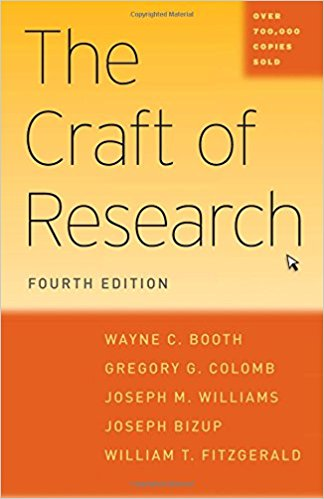
\includegraphics[scale=0.24]{../Figures/cover.jpeg}}
\logo{
\includegraphics[scale=0.1]{../Figures/mmilogo.png}}

\begin{document}

	\begin{frame}
	  \titlepage
	\end{frame}

% Problem definitons
\section{Introduction}

	\begin{frame}{Problem}
		
		\begin{itemize}
		  \item A deep network for object segmentation.  
		  \item \justifying This network has 5 two-by-two max-pooling layer, each of which downsamples its input by factor two. 
		\end{itemize}
		
	\end{frame}
	%next slide
	

	
%References
\section{References}
	%next slide
	\begin{block}{References}
	\end{block}
	\bibliography{./References/ref.bib}
	\bibliographystyle{ieeetr}

\end{document}